\documentclass[../views.tex]{subfiles}

\begin{document}

De physical view, te zien in \autoref{fig:physical_view}, omschrijft welke apparaten er gebruikt worden en hoe ze met elkaar communiceren \parencite{architectural_blueprints}. Het lijkt wellicht abstract, omdat de blokken (``Apparaten'', zie \autoref{fig:physical_view_legend}) geen labels bevatten. Dit is echter niet het geval. Er wordt inderdaad niet gespecificeerd welke programma's er op het apparaat draaien; dit is buiten de scope van de view. Uit de view is echter op te maken dat het blok waar een pijl naar zichzelf wijst de server, database en collector draait. De collector communiceert namelijk met de API op hetzelfde apparaat. Van dat apparaat moeten immers ook de specificaties verzameld worden. Er is ook een bidirectionele communicatielijn bij datzelfde blok. Dat is de API en de database die met elkaar communiceren. De andere apparaten draaien collectors of het dashboard; beide communiceren met de API, dus dit verschil is niet te onderscheiden in het diagram. Verder zullen in de praktijk meer dan vijf apparaten gebruikt worden, maar dit diagram is slechts een voorbeeld van hoe het eruit zou kunnen zien.

\begin{figure}[ht]
  \centering
  \fbox{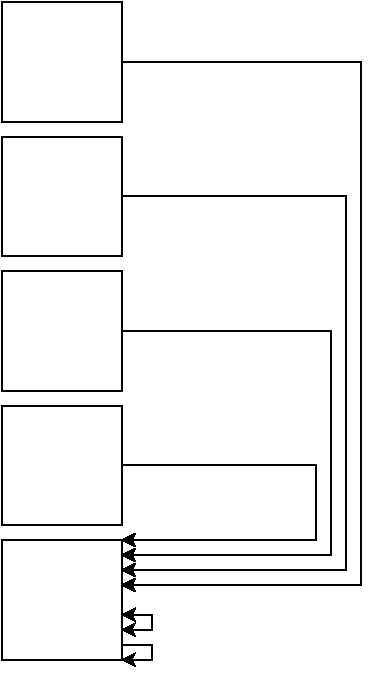
\includegraphics{assets/images/drawio/physical view.pdf}}
  \caption{De physical view.}
  \label{fig:physical_view}
\end{figure}

\begin{figure}[ht]
  \centering
  \fbox{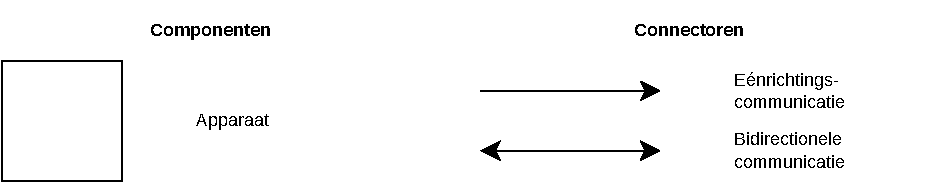
\includegraphics[width=0.95\textwidth]{../assets/images/drawio/physical view legend.pdf}}
  \caption{Legenda voor \autoref{fig:physical_view}.}
  \label{fig:physical_view_legend}
\end{figure}

\end{document}
